\documentclass[border=1cm,10pt]{standalone}

% I only need the arrows for this one.
\usepackage{tikz}
\usetikzlibrary{arrows}
\usetikzlibrary{decorations.pathmorphing}
\usetikzlibrary{decorations.markings}
\usetikzlibrary{trees}

\begin{document}

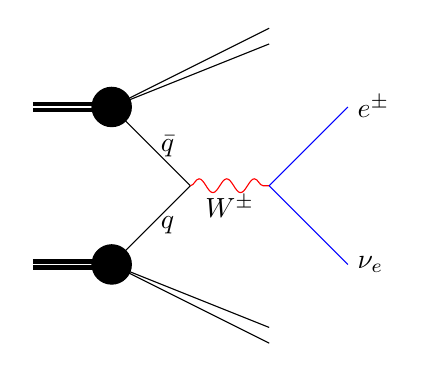
\begin{tikzpicture}[
  proton/.style={double, ultra thick},
  boson/.style={decorate, decoration={snake}, draw=red},
  lepton/.style={draw=blue},
  quark/.style={draw=black},
  gluon/.style={decorate, draw=magenta, decoration={coil,amplitude=4pt, segment length=5pt}} 
]

% Draw the incoming protons
\draw[proton] (0,1) -- (1,1) ;
\draw[proton] (0,3) -- (1,3) ;

% Draw the quarks
\draw[quark] (1,1) -- (2,2) node[midway,below,right] {$q$} ;
\draw[quark] (1,3) -- (2,2) node[midway,above,right] {$\bar{q}$} ;

% Draw the boson
\draw[boson] (2,2) -- (3,2) node[midway,below] {$W^{\pm}$} ;

% Draw the lepton and neutrino
\draw[lepton] (3,2) -- (4,3) node[right] {$e^{\pm}$} ;
\draw[lepton] (3,2) -- (4,1) node[right] {$\nu_e$} ;

% Draw the other stuff
\draw[quark] (1,1) -- (3,0) ;
\draw[quark] (1,1) -- (3,0.2) ;
\draw[quark] (1,3) -- (3,4) ;
\draw[quark] (1,3) -- (3,3.8) ;

% Draw the blobs
\filldraw (1,1) circle (.25);
\filldraw (1,3) circle (.25);

\end{tikzpicture}

\end{document} 
